\documentclass{article}\usepackage[]{graphicx}\usepackage[]{xcolor}
% maxwidth is the original width if it is less than linewidth
% otherwise use linewidth (to make sure the graphics do not exceed the margin)
\makeatletter
\def\maxwidth{ %
  \ifdim\Gin@nat@width>\linewidth
    \linewidth
  \else
    \Gin@nat@width
  \fi
}
\makeatother

\definecolor{fgcolor}{rgb}{0.345, 0.345, 0.345}
\newcommand{\hlnum}[1]{\textcolor[rgb]{0.686,0.059,0.569}{#1}}%
\newcommand{\hlstr}[1]{\textcolor[rgb]{0.192,0.494,0.8}{#1}}%
\newcommand{\hlcom}[1]{\textcolor[rgb]{0.678,0.584,0.686}{\textit{#1}}}%
\newcommand{\hlopt}[1]{\textcolor[rgb]{0,0,0}{#1}}%
\newcommand{\hlstd}[1]{\textcolor[rgb]{0.345,0.345,0.345}{#1}}%
\newcommand{\hlkwa}[1]{\textcolor[rgb]{0.161,0.373,0.58}{\textbf{#1}}}%
\newcommand{\hlkwb}[1]{\textcolor[rgb]{0.69,0.353,0.396}{#1}}%
\newcommand{\hlkwc}[1]{\textcolor[rgb]{0.333,0.667,0.333}{#1}}%
\newcommand{\hlkwd}[1]{\textcolor[rgb]{0.737,0.353,0.396}{\textbf{#1}}}%
\let\hlipl\hlkwb

\usepackage{framed}
\makeatletter
\newenvironment{kframe}{%
 \def\at@end@of@kframe{}%
 \ifinner\ifhmode%
  \def\at@end@of@kframe{\end{minipage}}%
  \begin{minipage}{\columnwidth}%
 \fi\fi%
 \def\FrameCommand##1{\hskip\@totalleftmargin \hskip-\fboxsep
 \colorbox{shadecolor}{##1}\hskip-\fboxsep
     % There is no \\@totalrightmargin, so:
     \hskip-\linewidth \hskip-\@totalleftmargin \hskip\columnwidth}%
 \MakeFramed {\advance\hsize-\width
   \@totalleftmargin\z@ \linewidth\hsize
   \@setminipage}}%
 {\par\unskip\endMakeFramed%
 \at@end@of@kframe}
\makeatother

\definecolor{shadecolor}{rgb}{.97, .97, .97}
\definecolor{messagecolor}{rgb}{0, 0, 0}
\definecolor{warningcolor}{rgb}{1, 0, 1}
\definecolor{errorcolor}{rgb}{1, 0, 0}
\newenvironment{knitrout}{}{} % an empty environment to be redefined in TeX

\usepackage{alltt}

\title{Data Visualization Assignment: Analyzing Data Science Salaries}
\author{Prashamsa Rijal \\ Student Number: 23140743\\Total Word Count: 985 \\ June 12, 2024}

\usepackage{graphicx}
\usepackage{amsmath}
\usepackage{amssymb}
\usepackage{hyperref}
\usepackage{float}
\usepackage{booktabs}
\usepackage{tabularx}
\usepackage{subcaption}
\usepackage{array}
\usepackage{caption}
\usepackage{xcolor}
\usepackage{tikz}
\usepackage{pgfplots}
\pgfplotsset{compat=1.18}
\usetikzlibrary{patterns}
\IfFileExists{upquote.sty}{\usepackage{upquote}}{}
\begin{document}

\maketitle

\newpage
\tableofcontents
\newpage
\listoffigures

\newpage
\section*{Abstract}
\addcontentsline{toc}{section}{Abstract}

The "Latest Data Science Salaries" dataset provides valuable insights into the compensation trends and variations in the field of data science from 2020 to 2024. This dataset encompasses a comprehensive collection of salary information from various industries, organizations, and geographic regions, enabling data professionals, researchers, and organizations to analyze and understand the prevailing salary landscape in the data science domain during this four-year period. By examining this dataset, one can gain a deeper understanding of the factors influencing data science salaries, such as job roles, experience levels, educational backgrounds, and geographical locations.

The dataset serves as a valuable resource for individuals seeking career guidance, companies aiming to benchmark their compensation strategies, and researchers investigating the evolving dynamics of the data science job market.

\newpage
\section{Introduction}
\subsection{Summarise}
This report is based on analyzing data science salaries from 2020 to 2024. The dataset includes detailed information on various job roles, experience levels, expertise levels, salaries, company characteristics, and geographical locations. The aim is to provide a comprehensive understanding of the salary trends and factors affecting compensation in the data science field.

The report is designed for readers with a medium level of understanding of data analysis and visualization. Additionally, some advanced topics are included for more experienced readers. The report addresses several key questions and provides conclusions based on the dataset.

\subsection{Highlight}
Overall, there are several interesting observations in this report:
\begin{itemize}
    \item Trends in salary growth over the four-year period.
    \item The impact of job roles and experience levels on salaries.
    \item Regional variations in data science compensation.
    \item The influence of company size and industry on salary levels.
\end{itemize}

These highlights provide a snapshot of the key findings from the dataset. Different readers may find different aspects more interesting, reflecting the diversity of perspectives in the field of data science.

\subsection{Aim}
The aim of this report is to explore and answer some of the most common questions regarding data science salaries. It investigates whether certain factors such as job role, experience level, educational background, and geographical location significantly impact compensation.

Another important goal is to dispel common misconceptions about data science salaries and provide a data-driven perspective on the job market dynamics.

\subsection{Achievements}
This report offers answers to several popular questions regarding data science salaries. It includes visualizations and analyses that map out salary distributions across different regions, identify the most lucrative job roles, and track salary changes over time.

Some theories about factors influencing salaries are confirmed, while others are challenged based on the data. For example, the analysis may show that experience level has a more significant impact on salary than educational background, or that salaries are higher in certain regions regardless of company size.

\subsection{Organised}
The structure of this report is as follows:
\begin{enumerate}
    \item Title
    \begin{enumerate}
        \item Subtitle (if applicable)
        \item Description
        \item Graphs (graphs are on their own page)
    \end{enumerate}
\end{enumerate}

This organization ensures that the information is presented in a logical and easy-to-follow manner, allowing readers to efficiently navigate through the various sections and find the insights they are most interested in.


\newpage
\section{Motivation and Objectives}
\subsection{Motivation}
The motivation behind this report stems from the growing interest in the field of data science and the increasing demand for data science professionals. Understanding salary trends and the factors that influence compensation is crucial for both job seekers and employers. This dataset, containing 3300 rows and 11 columns, offers a comprehensive overview of the salary landscape in data science from 2020 to 2024, making it an invaluable resource for detailed analysis and insights.

\subsection{Description of Selected Data}
The "Latest Data Science Salaries" dataset provides detailed information on various aspects of data science jobs. The dataset contains 3300 rows and includes the following 11 columns:
\begin{itemize}
    \item Job Title
    \item Employment Type
    \item Experience Level
    \item Expertise Level
    \item Salary
    \item Salary Currency
    \item Company Location
    \item Salary in USD
    \item Employee Residence
    \item Company Size
    \item Year
\end{itemize}
This extensive dataset enables a thorough analysis of the various factors that impact salaries in the data science field.

\subsection{Objectives}
The primary objective of this report is to analyze the "Latest Data Science Salaries" dataset to uncover trends and patterns in data science compensation. Specifically, it aims to identify the most significant factors influencing salaries, examine salary evolution over the four-year period, provide insights into regional variations, and offer data-driven conclusions to dispel common misconceptions about data science salaries.

\newpage
\section{Questions about Dataset}


\newpage
\section{Experimental Results}
\subsection{Salary Comparision of Data Scientists and Data Engineers based on expertise levels in the United States}
\textbf{This visualization explores the relationship between expertise level and salary for Data Scientists and Data Engineers in the United States. As the expertise level is good the salry is seen to be improved as well in both of the cases.While comparing the Data Scientist Job is seemes to have high income in case of expert and intermediate expertise.} 

\begin{knitrout}
\definecolor{shadecolor}{rgb}{0.969, 0.969, 0.969}\color{fgcolor}
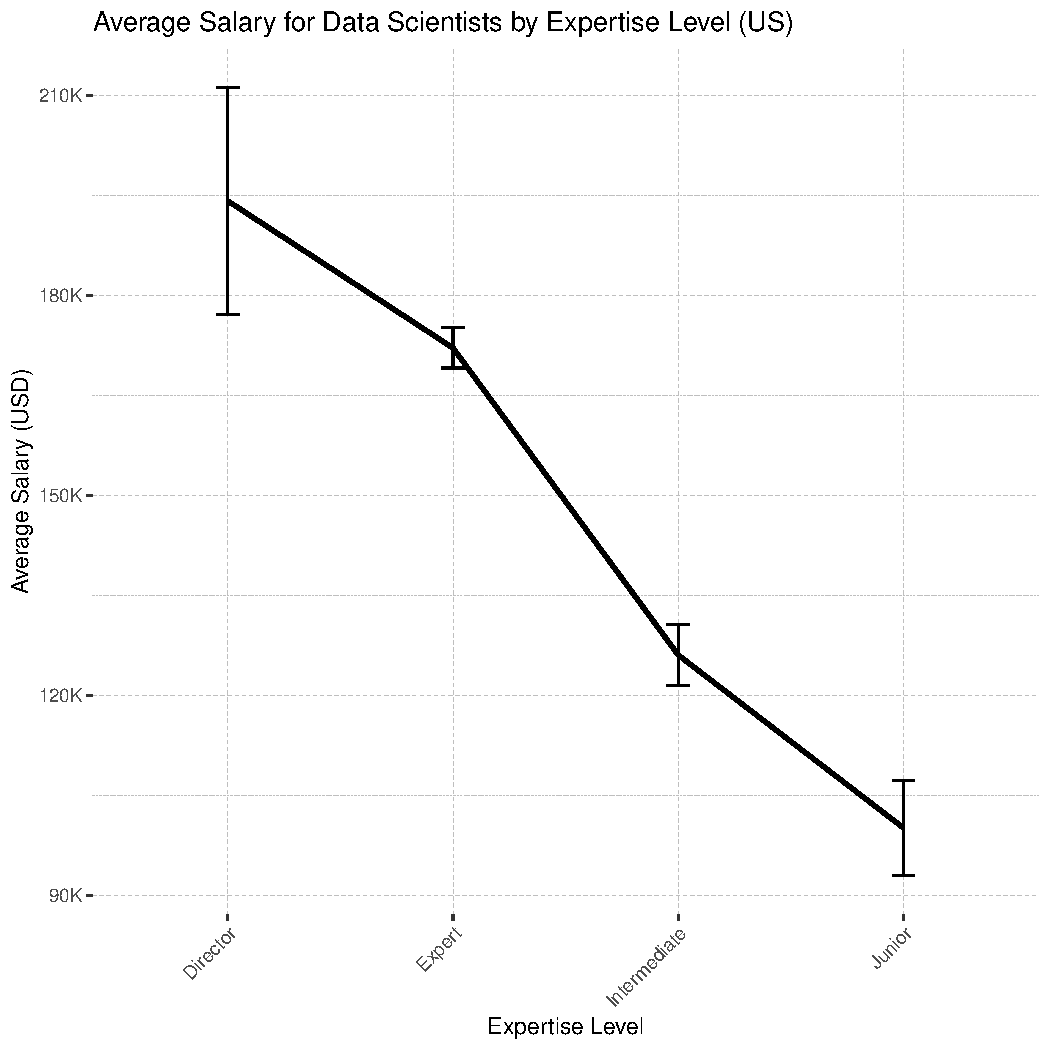
\includegraphics[width=\maxwidth]{figure/unnamed-chunk-2-1} 

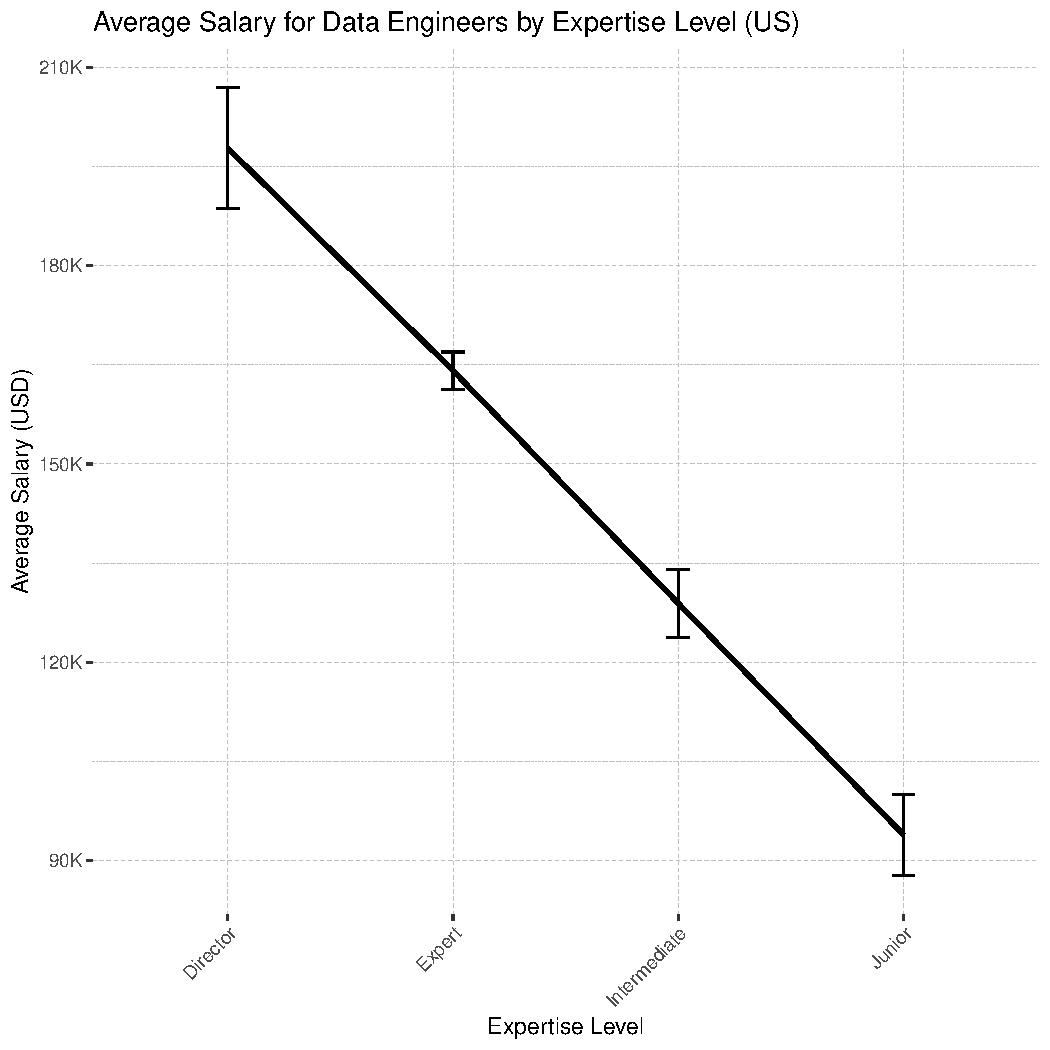
\includegraphics[width=\maxwidth]{figure/unnamed-chunk-2-2} 

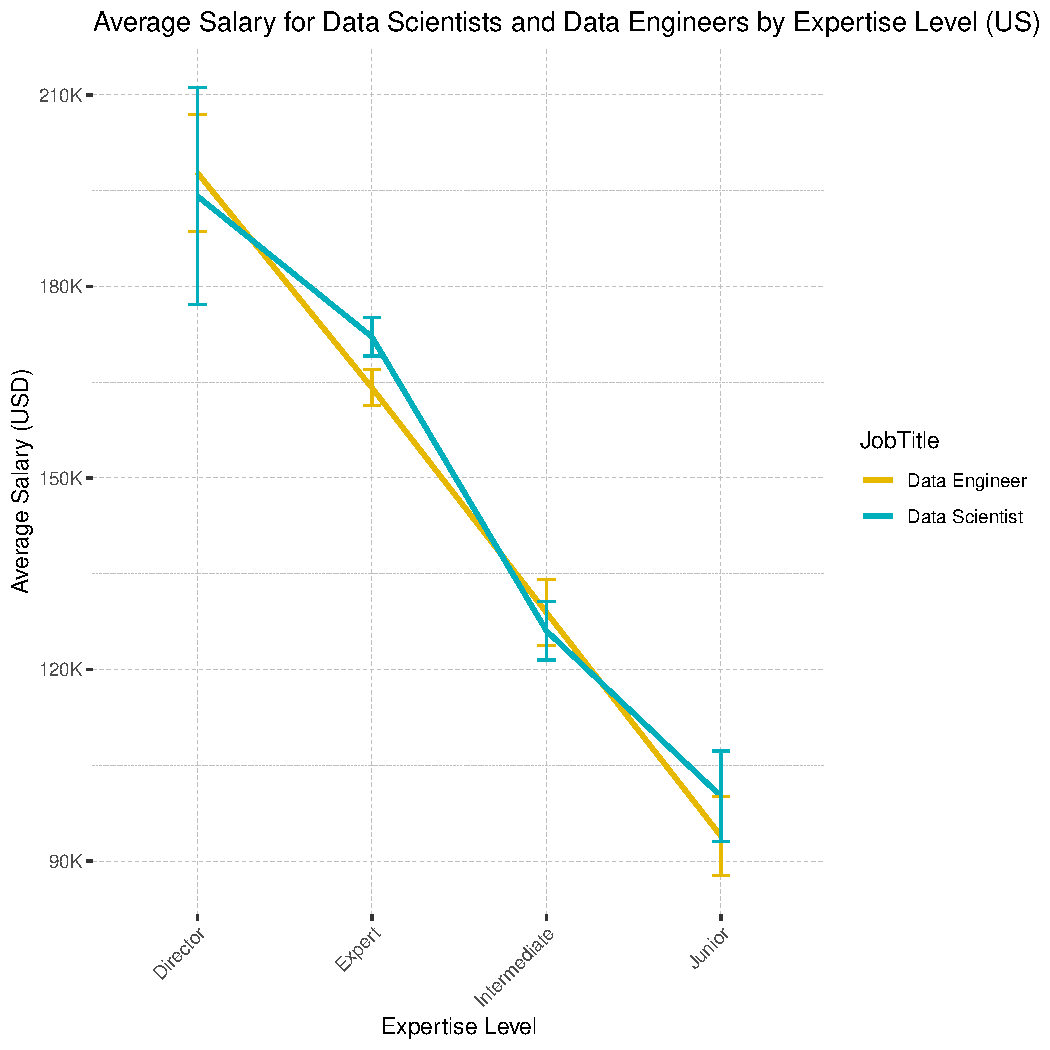
\includegraphics[width=\maxwidth]{figure/unnamed-chunk-2-3} 
\end{knitrout}

\newpage
\subsection{Varaince of Salary in Different Employment Type}

\textbf{This visualization shows how much data professionals earn based on their experience and the type of work they do (full-time, part-time, etc.). The plots show that the people who do full time earn the highest if they are executive or mid level.In other cases(contract and freelance) the mid experience is the most earning. }

\begin{knitrout}
\definecolor{shadecolor}{rgb}{0.969, 0.969, 0.969}\color{fgcolor}
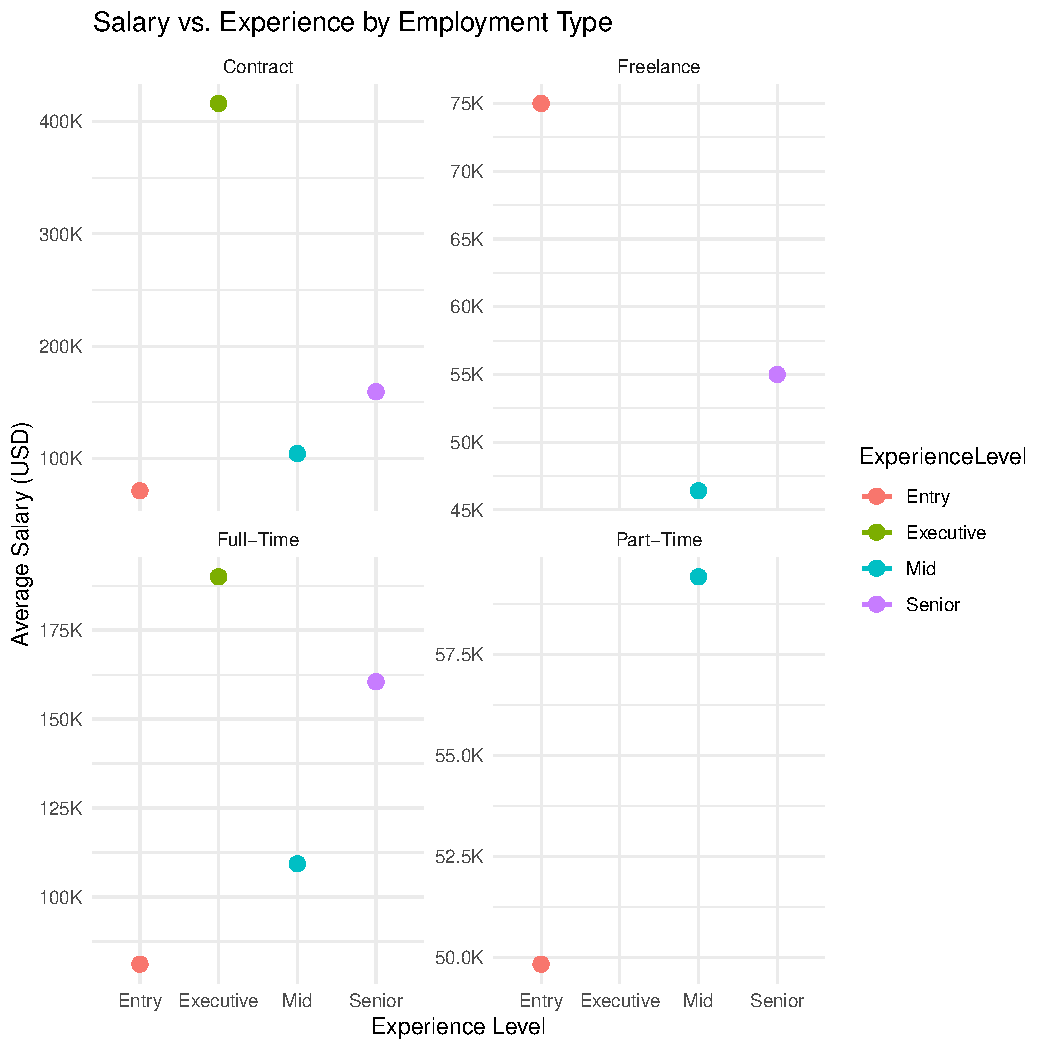
\includegraphics[width=\maxwidth]{figure/unnamed-chunk-3-1} 
\end{knitrout}

\begin{knitrout}
\definecolor{shadecolor}{rgb}{0.969, 0.969, 0.969}\color{fgcolor}
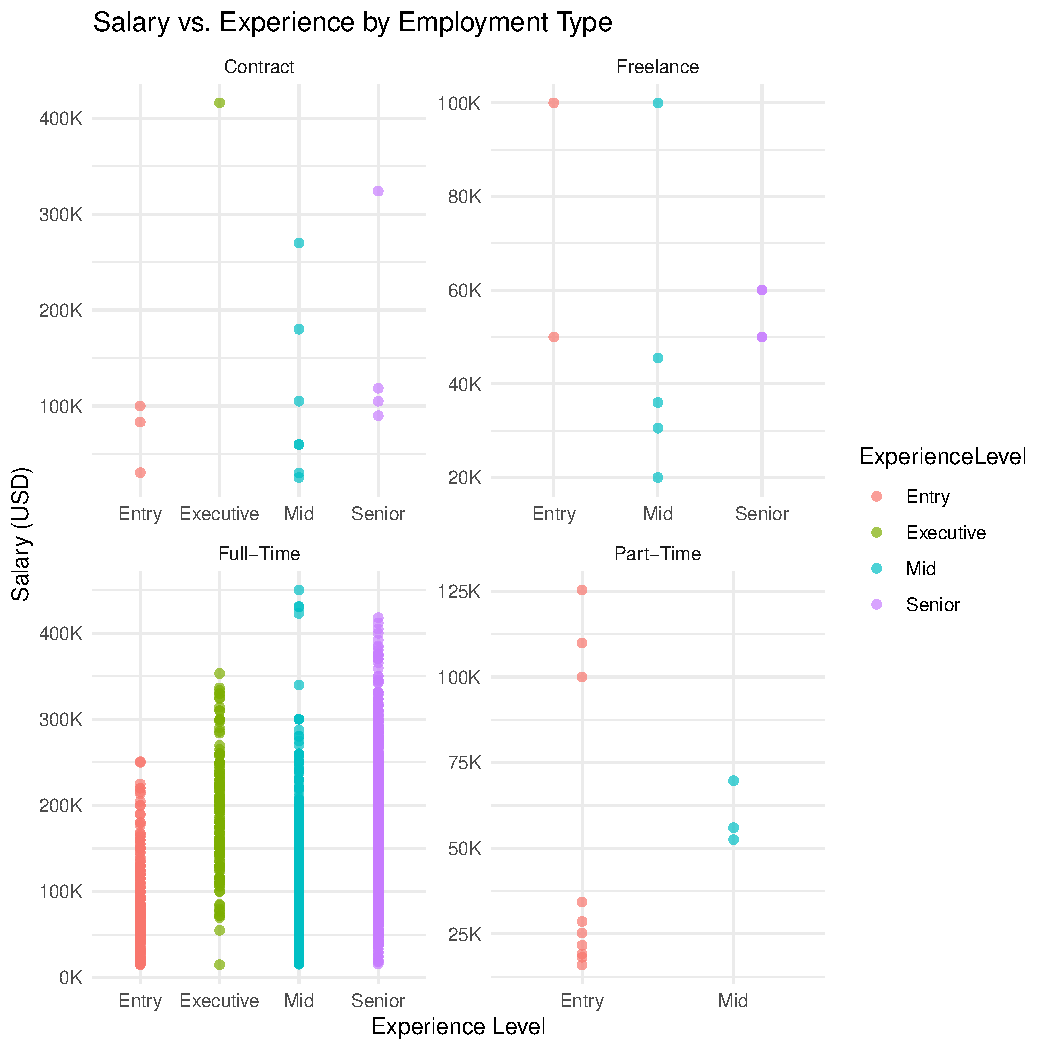
\includegraphics[width=\maxwidth]{figure/unnamed-chunk-4-1} 
\end{knitrout}

\newpage
\subsection{Salary Trend Over Time by Based on Experience Level}
\textbf{This visualization tracks how average salaries have changed over the years for data science professionals, grouped by how much experience they have. From visualization we can observe that there is increment in money over the time after 2021 in 2021 there was a fluctation in salary for all the job holders.} 

\begin{knitrout}
\definecolor{shadecolor}{rgb}{0.969, 0.969, 0.969}\color{fgcolor}
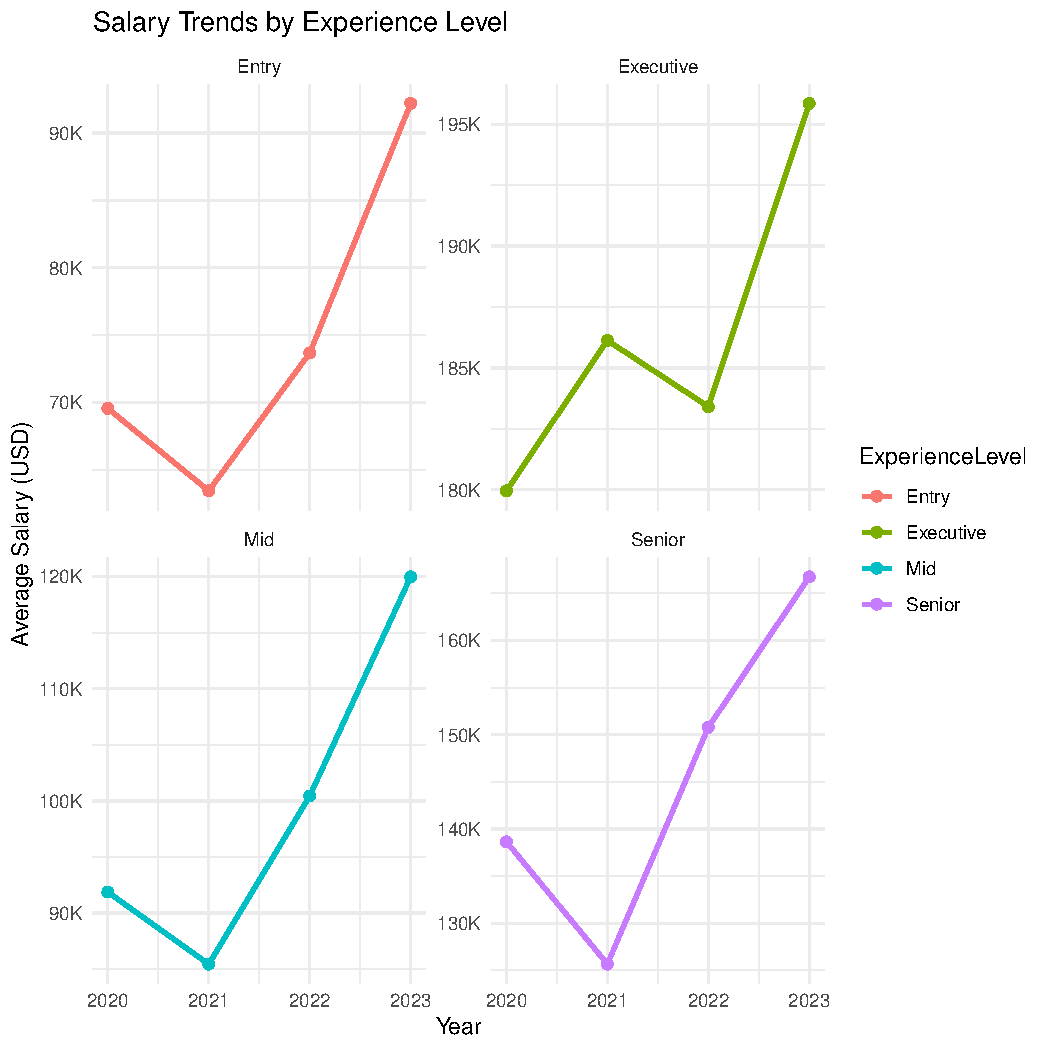
\includegraphics[width=\maxwidth]{figure/unnamed-chunk-5-1} 
\end{knitrout}


\newpage
\subsection{Change in company Size Over Time}
\textbf{This visualization shows how the number of data science companies of different sizes has changed over the years. The bar chart shows how many companies are in each size category for each year.We can see that medium sized company has increased alot compared to others over the year although at first there were more large companies. }

\begin{knitrout}
\definecolor{shadecolor}{rgb}{0.969, 0.969, 0.969}\color{fgcolor}
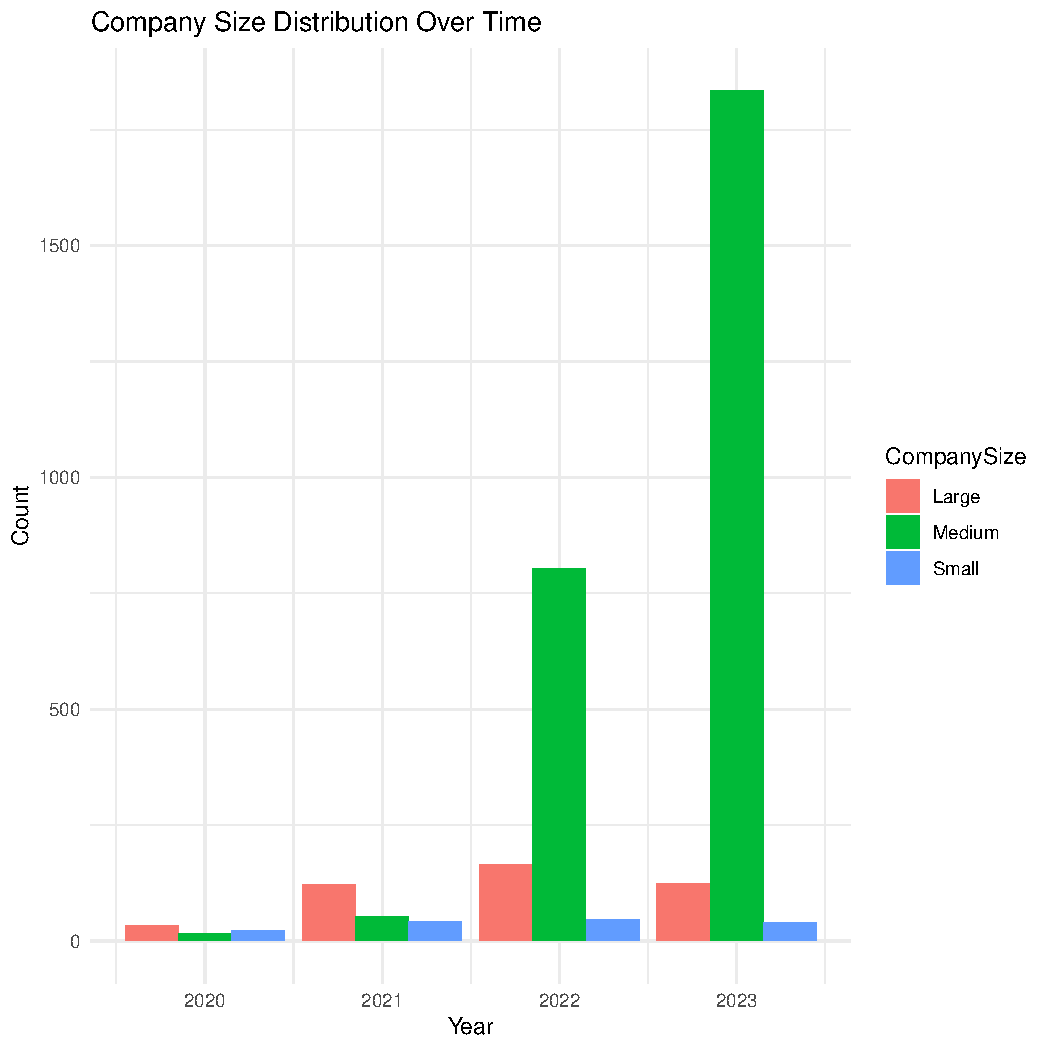
\includegraphics[width=\maxwidth]{figure/unnamed-chunk-6-1} 
\end{knitrout}


\newpage
\subsection{Salary Expectations accross different Jobs}
\textbf{This visualization shows how salaries for the 10 highest-paying data science job roles have changed over the years. Some jobs were highest paying for a year only then it was no more seen in other years whereas the one job that is seen from 2020 till 2023 is Director of Data Science.Comapred to 2022 the income has decreased for many of the job roles.} 

\begin{knitrout}
\definecolor{shadecolor}{rgb}{0.969, 0.969, 0.969}\color{fgcolor}
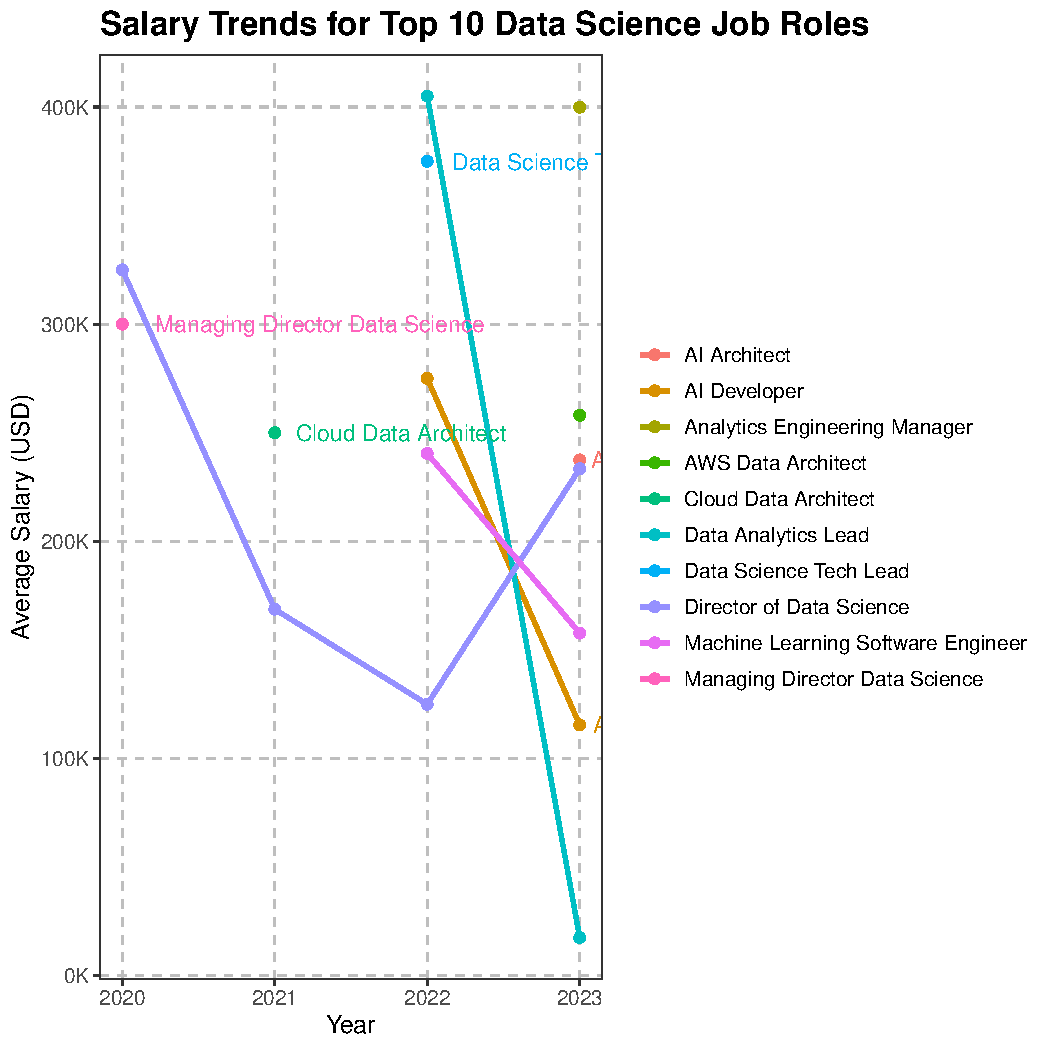
\includegraphics[width=\maxwidth]{figure/unnamed-chunk-7-1} 
\end{knitrout}

\begin{knitrout}
\definecolor{shadecolor}{rgb}{0.969, 0.969, 0.969}\color{fgcolor}\begin{kframe}


{\ttfamily\noindent\itshape\color{messagecolor}{FALSE `summarise()` has grouped output by 'JobTitle'. You can override using the\\FALSE `.groups` argument.}}\end{kframe}
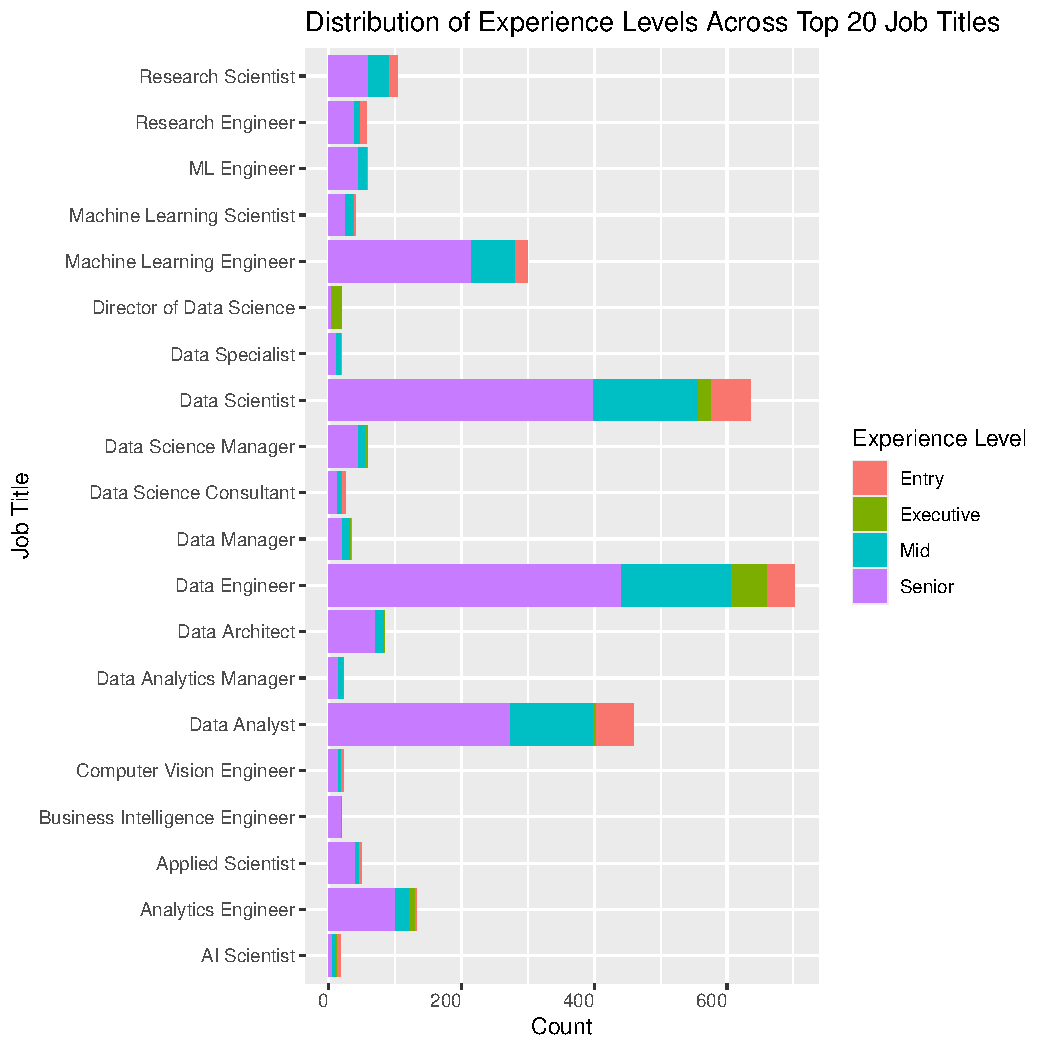
\includegraphics[width=\maxwidth]{figure/unnamed-chunk-8-1} 
\end{knitrout}




\newpage
\section{Summary}

\newpage
\section{References}
\addcontentsline{toc}{section}{References}
\begin{itemize}

\item {KaggleDataset2023}
Kaggle. (2023). Data Science Salaries 2023. Kaggle. Available at: https://www.kaggle.com/datasets/iamsouravbanerjee/data-science-salaries-2023 

\item {AIJobsNet2023}
AI-Jobs.net. (2023). Data Science Salaries. Available at: https://ai-jobs.net/ 

\item {Ramachandran2024}
Ramachandran, K. K. (2024). Data Science in the 21st Century: Evolution, Challenges, and Future Directions. *International Journal of Business and Data Analytics*, 1(1), 1-15. 
\end{itemize}

\end{document} 
